\documentclass[10pt]{article}
\usepackage{graphicx}
\usepackage{algorithm}
\usepackage{hyperref}

\usepackage{algorithmic}
% \usepackage{gensymb}
\usepackage{fullpage}
\usepackage{float}
\usepackage{subcaption}

\parskip 0.05in
\begin{document}
\title{\bf Can we predict fire with weather data?}
\author{Harsh (hp444), Yi Yao (yy899), Murali (mt788)}
\maketitle

\begin{abstract}
In this report, we explore the idea od using the weather parameters such as
temperature, pressure, etc to predict if a wild fire may occur. The datasets in
use are the \textit{Wild Fires Dataset} and the \textit{Weather Dataset}.
The datasets were combined to use realistic weather features as inputs along
with binary \textit{fire/no fire} output. This is clearly a binary
classification problem and a very imbalanced one. Dealing with the imbalance is
the highlight of this report. We use precision and recall metrics to form the
dataset. We attempted to use algorithms like \textit{SVM, XGBoost} and also
autoML (\textit{TPOT}). We show our preliminary results on how we deal with
imbalance and also how we plan to work on this issue in the next half of the
semester.\par
\end{abstract}

\section{Introduction}

The weather has literally been the \textbf{hot topic} of discussion in recent
times. One aspect of weather data is that, when it is combined with other data
sets, it can be used to predict a lot of different aspects related to society.
For example, one interesting aspect could be how does the traffic condition
changes based on the weather in a particular city or if there is a correlation
between crime rates and weather conditions. In this project, we are trying to
address a more important issue of predicting wildfires in different cities
based on weather conditions. Since the future weather data is readily available
these days, a good model would help predict these wildfires in advance and take
necessary precautions to completely avoid it. This would help avoid
human/wildlife loss.\par

\section{Data Statistics}

Here is a quick look into the data that we're working with. Table 1 shows the
statistics of the weather data and Table 2 shows the statistics of the fire
data.\par

\begin{table}[H]
    \centering
    \begin{minipage}[t]{0.45\textwidth}
        \caption{Weather Data Statistics}
        \begin{tabular}{c c c}
            \hline
            Elements & \# \\ % inserts table
            %heading
            \hline
                Cities & 36 \\
                Features/city & 9 \\
                Total Samples & 1.63 million \\
                Samples/city & 45 thousand 
                
        \end{tabular}
    \end{minipage}
    \begin{minipage}[t]{0.45\textwidth}
        \caption{Wild Fire Data Statistics}
        \begin{tabular}{c c}
            \hline
            Elements & \# \\ % inserts table
            %heading
            \hline
            Cities & 36 \\
            Features/city & 9 \\
            Total Samples & 1.63 million\\
        \end{tabular}
    \end{minipage}
\end{table}
\section{Data Cleaning/ Data Exploration/
\href{https://leafyao8621.github.io/firevisualization.github.io/}
{Data Viz Website}}
First, we combined both the datasets to arrive at one single table containing
the weather features and simply attributing fire/no fire column. This was not
straight forward because the fire data had latitude and longitude for refernce
while weather data had cities. The first challenge was to identify the slack to
allocate cities to the co-ordinates. We gave a $1^\circ$ (which is roughly
100 km) which was a safe distance to associate with the city weather data.
After this, we had to parse the tables with weather features and the binary
fire/no fire feature. This resulted in 10 features in X space and one feature
in y space. We had to perform one-hot encoding for one of the parameters which
was weather description because of which we were left with 33 features at the
end.\par

In San Fransisco, the number of fires in the set was 1260 and the number of
no-fires is roughly 43 thousand. This would cause issues with overfitting.
Using the precision and recall metrics, we actually find that the number of
data points where the tradeoff occurs is with 1400 negative examples with 1400
positive samples or in some sense almost equal number of positive and negative
examples. Figure 1(a) and Figure 1(b) show the number of negative examples
needed to ensure tradeoff between precision and recall. Also, we know that
California is burning at the moment, Figure 1(d) shows the distribution of
number of fires in all cities we have data for grouped by hour where fires
where actually reported. If you want to look at fires in the cities we are
covering, Figure 1(c) shows a screen shot of one instant of time. The animation
showing fires over time is hosted on \textit{Github}.
\textit{Follow this
\href{https://leafyao8621.github.io/firevisualization.github.io/}{link}
and please allow for sometime for the website to load}.\par

\begin{figure}[H]
    \caption{}
    \centering
    \begin{subfigure}[t]{0.45\textwidth}
        \caption{}
        \centering
        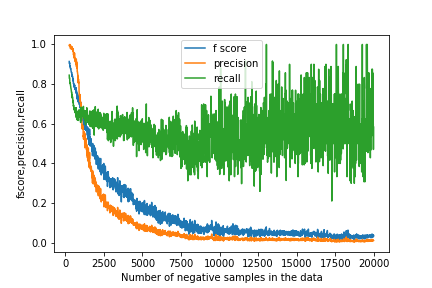
\includegraphics[width=0.9\textwidth]{image.png}
    \end{subfigure}
    \begin{subfigure}[t]{0.45\textwidth}
        \caption{}
        \centering
        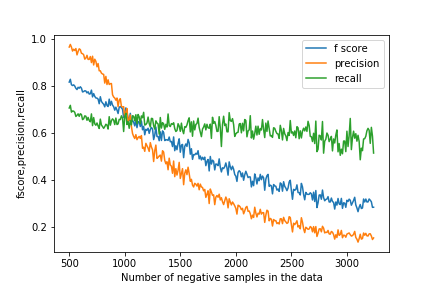
\includegraphics[width=0.9\textwidth]{image1.png}
    \end{subfigure}
    \begin{subfigure}[t]{0.45\textwidth}
        \caption{}
        \centering
        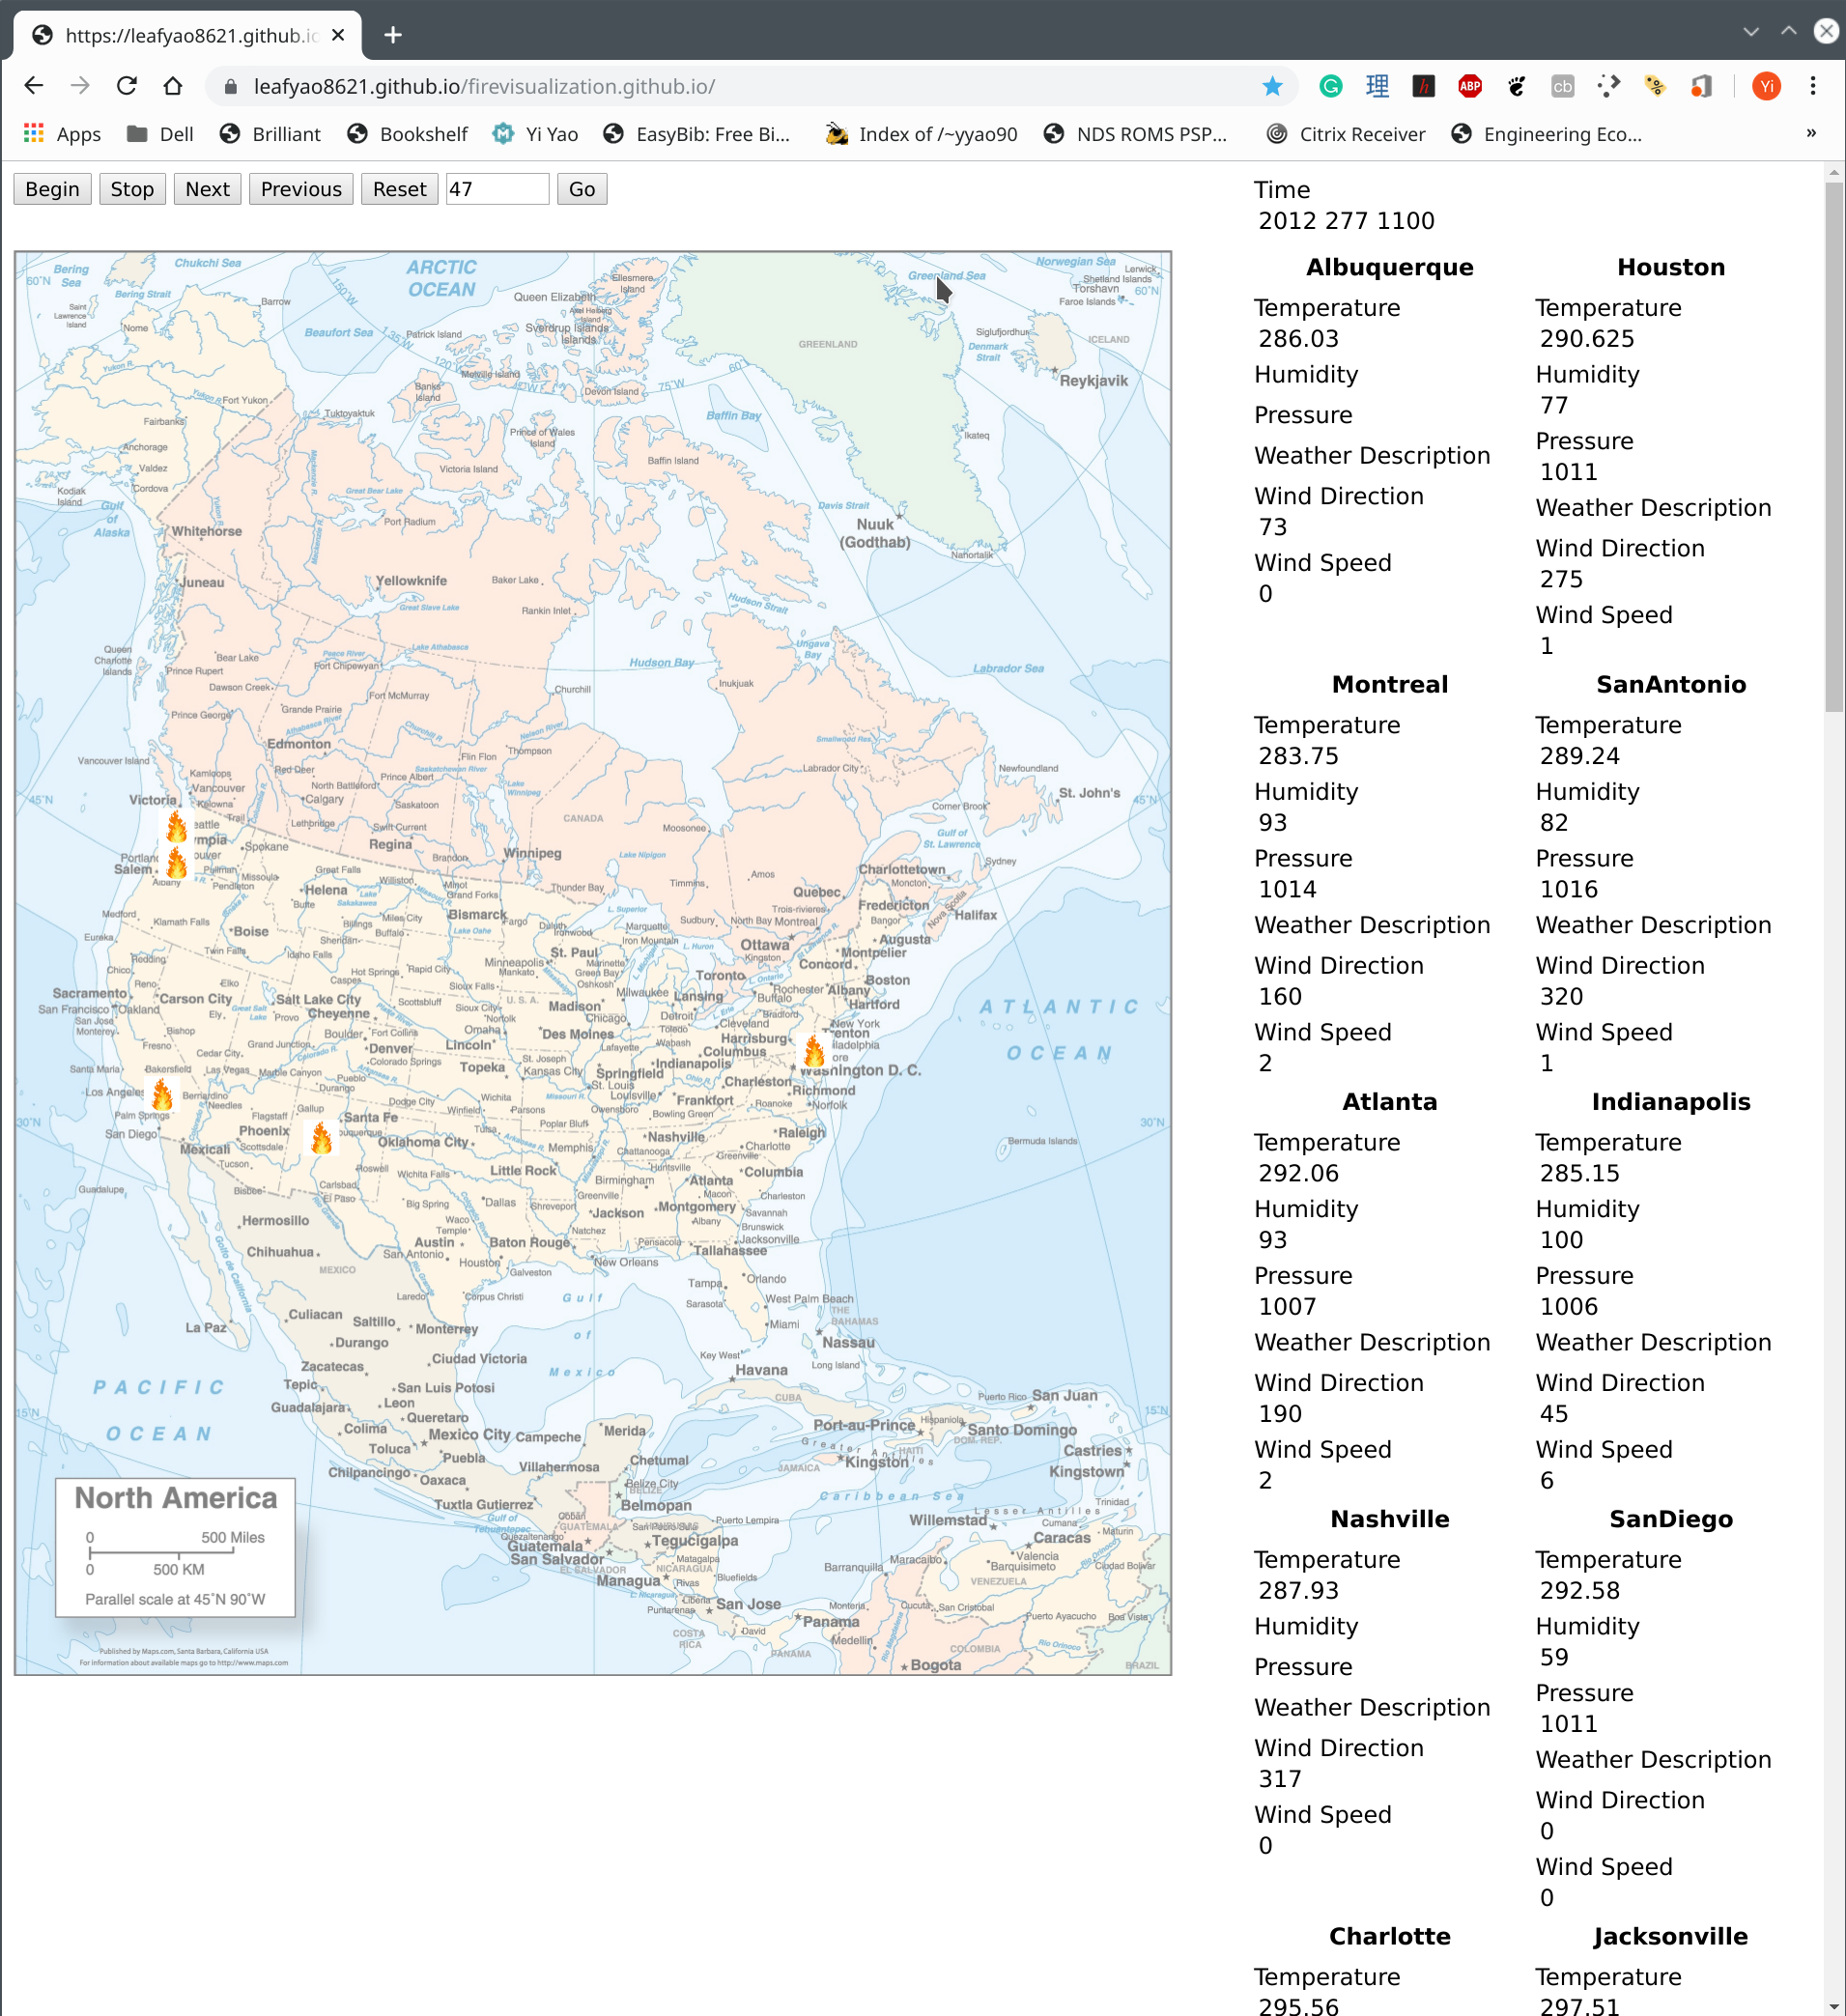
\includegraphics[width=0.5\textwidth]
        {../../visualization/screenshot.png}
    \end{subfigure}
    \begin{subfigure}[t]{0.45\textwidth}
        \caption{}
        \centering
        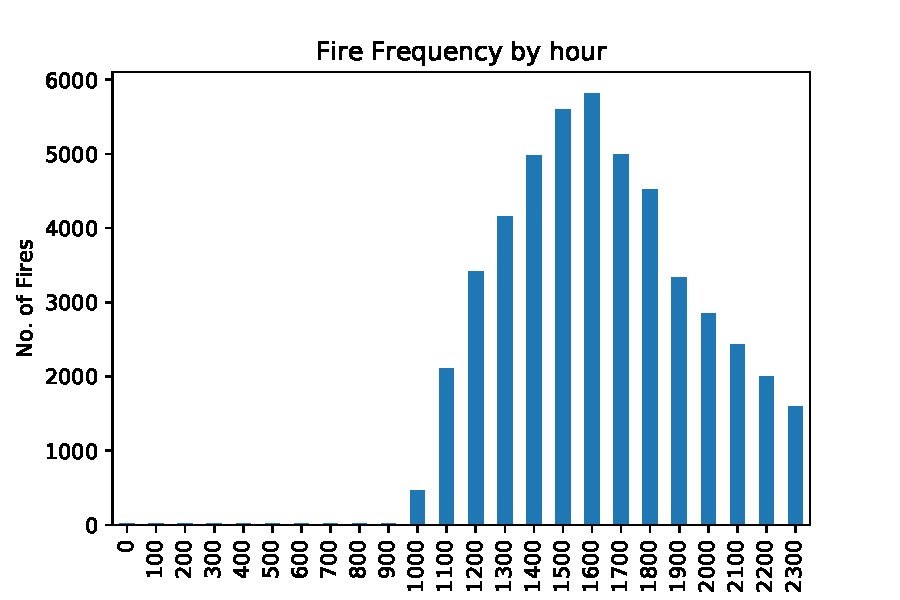
\includegraphics[width=0.9\textwidth]{Allfire.pdf}
    \end{subfigure}
\end{figure}

\section{Data Analysis}

Our goal is to construct city-specific models to predict fire with weather
data. First of all, we randomly sampled 20\% of the data points from a
particular city with value 1 for the Fire variable, and sampled the same
\textbf{number} of data points from that city with value 0 for the Fire
variable to form a \textbf{balanced} test set. The models were then trained 
on the remaining data points where we again constructed a \textbf{balanced}
data set by combining the ramining data points with 1 for fire and a
sample with the same \textbf{number} of data points from the
remaining data points with 0 for Fire. Meta parameters were selected by
comparing 5-fold cross-validtion score on the training data set.\par

We decided to use two ensemble learning models, namely XGBoost and
Random Forest, as well as a linear model, namely Soft-Margin SVM with the RBF
(Radial Basis Function) kernel. On top of
this, we also ventured using automl framework TPOT. The following table
summarises the results for two cities.\par


\begin{table}[H]
    \caption{SanFrancisco}
    \centering
    \begin{tabular}{|r|r|r|r|r|r|r|r|r|}
        \hline
        Classifier &Meta Parameter
        &\multicolumn{4}{|r|}{Training}
        &\multicolumn{2}{|r|}{Test}\\
        \hline
        &n\_estimators
        &acc
        &bal\_acc
        &prec
        &rec
        &acc
        &bal\_acc
        &prec
        &rec\\
        \hline
        XGBClassifier &96 &0.0000 &0.6404 &0.0000 &0.0000
        &0.6766 &0.6790 &0.7341 &0.6584\\
        \hline
        RandomForestClassifier &41 &0.0000 &0.6632 &0.0000 &0.0000
        &0.7063 &0.7089 &0.7619 &0.6857\\
        \hline
    \end{tabular}
\end{table}


\begin{table}[H]
    \caption{97}
    \centering
    \begin{tabular}{|r|r|r|r|}
        \hline
        Classifier &Meta Parameter &Training Accuracy
        &Test Accuracy\\
        \hline
        &n\_estimators &\multicolumn{2}{|r|}{}\\
        \hline
        XGBClassifier &Atlanta &0.7077 &0.6982\\
        \hline
        RandomForestClassifier &50 &0.7248 &0.7124\\
        \hline
        &C &\multicolumn{2}{|r|}{}\\
        \hline
        SVC &0.5000 &0.6415 &0.6580\\
        \hline
    \end{tabular}
\end{table}


From the summaries, we discovered that the models perform similarly on training
and testing data sets which indicates that we might have alleviated
overfitting, but the accuracy scores themselves are not high. Our next step
will be improving accuracy scores while avoiding overfitting.\par

\section{Work for the upcoming term}
\subsection{Bootstrapping}
To avoid overfitting problem, we may try out the following pseudocode hoping to
solve the problem:
\begin{algorithm}
    \caption{Avoid Overfit using our version of Bootstrap}
    \begin{algorithmic}[lt]

        \STATE DPos $\gets$ Positive data and DNeg $\gets$ Negative
        data
        \FOR{Number of Iterations}
        \STATE Sample negative data in equal proportion to available positive
        data
        \STATE Fit the data and store the weights
        \ENDFOR
        \STATE Average the weights to get an averaged model
        \STATE Test this model on a new and unseen data for validation
        \REQUIRE Changing the ratio of sampling in the dataset to average
        different models
        \STATE Test this model on a new and unseen data for validation
    \end{algorithmic}
\end{algorithm}

\subsection{Feature Engineering}
Feature Engineering plays a key role in cases like ours where our data is very
restrictive within certain ranges. We plan to use different feature
transformations like exponentials, logarithms. Apart from this, we may also
explore into using different data available online for more feature information
related to fires and

\end{document}
